% tikzpic.tex
\documentclass[crop,tikz]{standalone}% 'crop' is the default for v1.0, before it was 'preview'
%\usetikzlibrary{...}% tikz package already loaded by 'tikz' option
\usepackage{amsmath,amsthm,amssymb,mathrsfs,amsfonts,dsfont}
\usetikzlibrary{plotmarks}

\begin{document}
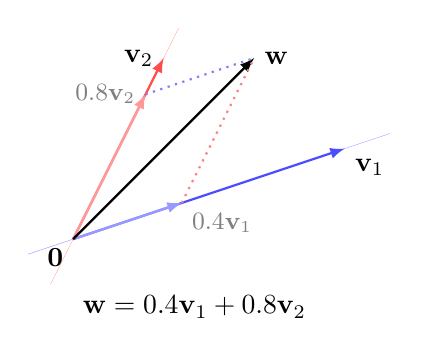
\begin{tikzpicture}[scale=1.15]
    \node[below left,xshift=0.0cm, yshift=0.0cm,black] at (0, 0) {$\mathbf{0}$};
    %%%%% v1
    \draw[-, ultra thin, blue!50] (-0.5,-0.167) --  (3.5, 1.167);
    \draw[-latex, thick, blue!70] (0,0) --  (3,1) node[below right, black] {$\mathbf{v}_1$};
    \draw[-latex, thick, blue!40] (0,0) --  (1.2,0.4) node[below right, gray] {\small $0.4\mathbf{v}_1$};
    %%%%% v2
    \draw[-, ultra thin, red!50] (-0.25, -0.5) --  (1.167, 2.334);
    \draw[-latex, thick, red!70] (0,0) --  (1, 2) node[left, black] {$\mathbf{v}_2$};
    \draw[-latex, thick, red!40] (0,0) --  (0.8,1.6) node[left, gray] {\small $0.8\mathbf{v}_2$};
    %%%%% w
    \draw[-latex, thick, black] (0,0) --  (2, 2) node[right, black] {$\mathbf{w}$};
    \draw[dotted, thick, blue!50] (0.8, 1.6) --  (2,2);
    \draw[dotted, thick, red!50] (1.2, 0.4) --  (2,2);
    \node[right] at (0, -0.75) {$\mathbf{w} = 0.4\mathbf{v}_1 + 0.8\mathbf{v}_2$};
\end{tikzpicture}
\end{document}